\section{Fast scale-space context-sensitive features}
\label{sec: features}

%$3D$ medical image segmentation demands scalable, robust, high precision solutions. 
We revisit scale-space representations to craft fast, expressive, compactly parameterized features, as a simple alternative to the popular integral or Haar-like features \cite{viola2001rapid}.\\

\noindent
\textbf{Background: integral features.} Integral features are based on intensity averages within anisotropic cuboids offset from the point of interest \cite{criminisi2013regression}. Cuboid averages are computed in constant time by probing the value of a precomputed integral map at the cuboid vertices \cite{viola2001rapid}. For instance, $f(\brmx, \bm{\theta})\!\triangleq\!\sum_{x'\in\calC_2}\!I_{j_2}(x') - \sum_{x'\in\calC_1}\!I_{j_1}(x')$ computes the difference of responses in cuboids $\calC_1$ and $\calC_2$ of size $\bm{s_1}\eq(s_1^x,s_1^y,s_1^z)$ and $\bm{s_2}\eq(s_2^x,s_2^y,s_2^z)$, centered at offset locations $x+\bm{o}_1$ and $x+\bm{o}_2$, in distinct channels $I_{j_1}$ and $I_{j_2}$. Here $\bm{\theta}\eq(j_1,j_2,\bm{o}_1,\bm{o}_2,\bm{s}_1,\bm{s}_2)$ is a $14$-dimensional feature.\\

\noindent
\textbf{Proposed scale-space representation.} During node training, it is crucial for sufficiently strong 
weak-learners to be computable within the budget allocated to feature sampling and optimization. 
Therefore, reducing the feature parameterization while maintaining expressiveness is key. 
For integral features, the sophistication of probing anisotropic cuboids with a continuous range of edge lengths 
comes at a cost w.r.t. parametric complexity. We restrict ourselves to a small \textit{finite} range of \textit{isotropic} averages. We augment the original set of input channels with their smoothed counterparts under separable 
Gaussian filtering at scales $\sigma_1$, $\sigma_2$ etc. Given $s$ scales, $f(\brmx, \bm{\theta})\!\triangleq\!I_{j_2}(x+\bm{o}_2) - I_{j_1}(x+\bm{o}_1)$ computes the difference of responses in channels $j_\epsilon\,\text{mod}\,s$ at scales $j_\epsilon / s$ with offset $\bm{o}_\epsilon$ from voxel $x$ ($\epsilon\eq1,2$). Here $\bm{\theta}\eq(j_1,j_2,\bm{o}_1,\bm{o}_2)$ is an $8$-dimensional feature. 

A single point is probed for every $8$ cuboid vertices probed under integral features, as well as circumventing many boundary checks. For all practical purposes ($s=2,3$), \texttt{byte[]} storage of scale-space maps limits the memory 
overhead relative to integral maps (\texttt{short[]} storage).\\

\noindent
\textbf{Fast rotation invariant features.} We also illustrate (in Section~\ref{}) how to go beyond \textit{directional} context and account for natural local invariances with an example of fast, multiscale, approximately rotation invariant feature. Let $\phi_1\cdots\phi_{12}$ stand for the coordinates of an axis-aligned, centered icosahedron of radius $r$. Denoting by $\bm{\theta}\eq(j_1,j_2,r)$ the $3$-dimensional feature, $f(\brmx, \bm{\theta})\!\triangleq\! \text{Median}_{v=1}^{12} \vert I_{j_2}(x+\phi_v)\!-\!I_{j_1}(x)\vert$ gives a robust summary of intensity variations around point $x$. %Fig. \ref{fig: features} compares the feature impact on speed and accuracy to that of a directional line response introduced in \cite{zikic2012decision}. %Our implementation hard-codes $12$-array median computations for efficiency. We also impose $j_2 / s > j_1/s$ to mimic the intuition of coarser peripheral vision relative to the focus $x$ of interest.

%\begin{figure}
%\centering
%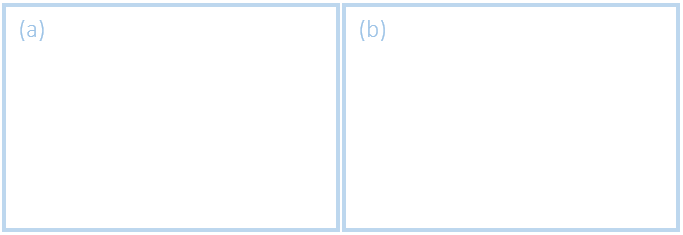
\includegraphics[width=1\columnwidth]{images/features_lead-illustration.png}
%\caption{(a) Accuracy vs. choice of feature for CVE (bar plot): baseline (Haar features) vs. baseline + line response vs. scale-space vs. scale-space + rotation-invariant. Mention total running time for each setting (either number or chart). (b) Average computation time for different feature types.}
%\label{fig: features}
%\end{figure}

% Dual thresholding can be mentionned somewhere in the TMI paper version

% Figures that I want to see:
% Accuracy vs. choice of feature for CVE (bar plot): baseline (Haar features) vs. baseline + line response vs. scale-space vs. scale-space + rotation-invariant. Small plots: a) total running time for each setting b) average computation time for different feature types.
